\documentclass[a4paper,twoside]{article}

\usepackage{epsfig}
\usepackage{subcaption}
\usepackage{calc}
\usepackage{amssymb}
\usepackage{amstext}
\usepackage{amsmath}
\usepackage{amsthm}
\usepackage{multicol}
\usepackage{xcolor}
\usepackage{pslatex}
\usepackage{hyperref}
\usepackage{apalike}
\usepackage{url}
\usepackage{booktabs}
\usepackage{SCITEPRESS}     % Please add other packages that you may need BEFORE the SCITEPRESS.sty package.


\begin{document}

\title{Evaluating early results in XXX}

\author{\authorname{Vladimir Ivanov\orcidAuthor{0000-000x-xxxx-xxxx}, Vitaly Romanov\orcidAuthor{0000-000x-xxxx-xxxx}, Giancarlo Succi\orcidAuthor{0000-0001-8847-0186}
}
\affiliation{\sup{1}Innopolis University, Russia}
\email{\{f.last\}@innopolis.ru}
}

\keywords{}

\abstract{
% \href{https://github.com/VitalyRomanov/method-embedding}{Github} | 
% \href{https://docs.google.com/document/d/1Xwn7RWtS1ORKu3fVV2NgVS7aHwsULMlYpalR0RiVq6Q/edit#heading=h.ajuwnh29h0tg}{Google Doc}
}

\onecolumn \maketitle \normalsize \setcounter{footnote}{0} \vfill

\section{\uppercase{Introduction}}
% \noindent 
Source code can be viewed as a form of natural language. Lately we see the rise of the approaches that try using advances in the area of Natural Language Processing to solve machine learning tasks for source code. One of the noteworthy applications of modeling source code is the source code search. In this application, a user can find a relevant code snippet using a natural language query. Such approaches do not even require the code to have any extra annotation or documentation. However, most of such approaches work on the level of the body of a single function, which, in most cases, is sufficient to understand the purpose of this function. However, learning algorithms still struggle to process sequences of actions that are common in source code. At the same time, current approaches proved to be quite successful in capturing co-occurrence statistics. For source code, such statistics can be extracted from global usage patterns on a package or inter-project levels. Our goal is to study how useful this global information is by posing this goal as an evaluation of machine learning tasks on graphs.
 
Source code describes the relationships between source code objects (SCOs), such as modules, functions, classes, variables, etc. Some information about these SCOs can be inferred from the package and inter-project level dependencies. A package contains information about the contextual similarity. The SCOs from the same package are likely to have a related purpose. The information about how particular SCOs are used in different projects can tell us which packages are often used together, and what are the common combinations of SCOs to be used together in various projects. On these levels of abstraction, one does not concern with the particular way an SCO is implemented and can learn useful insights about its purpose from merely observing the way it is used. Traditional NLP approaches are not suited to capture these kinds of relationships because they treat the input as a sequence of tokens. A structured representation of the source code is required instead.

The package and inter-project levels of abstraction are well represented using a graph. Such a graph can include different types of relationships, including call dependencies, type dependencies, import dependencies, variable usages, inheritance dependencies, and others. Because the relationships between SCOs are not constrained to the boundaries of particular functions, files, and even packages, such a graph captures global relationships, and, therefore, is a global graph. Global graph representation is an alternative approach to represent the source code besides other structures representations, such as abstract syntax trees (ASTs). We evaluate the usefulness of this global graph representation by solving different machine learning problems for source code. In this work, we aim at assessing what kind of information can be inferred from high-level inter-project global relationships between SCOs. Moreover, we look into the transferability of learned distributed representations for nodes in this graph to other problems. We purposefully do not consider the ASTs as their study was addressed in other works \cite{Alon2018}, \cite{Yahav2018}.

There are several papers that investigated what a model can learn from a particular source code representation. \cite{Alon2018a} used AST paths to predict the names of functions. \cite{Allamanis2017} used graph representation that relies on both global relationships and ASTs to find bugs. \cite{DeFreez2018} used an inter-procedural flow graph to find similar functions inside the Linux kernel source code. \cite{Raychev2015} used information about AST to predict variable names and types within a function. In contrast to these works, we focus on using only information about global relationships. 

Our contribution is the following
\begin{itemize}
    \item We introduce a source-graph-dataset that captures information about global relationships between over 100 Python packages;
    \item We evaluate the usefulness of a global graph on several machine learning tasks, including SCO name prediction, variable name usage prediction, API call sequence prediction. For our experiments we use Graph Neural Networks (GNNs);
    \item We evaluate the transferability of learned distributed representations of graph nodes by training additional models that try to predict different properties of SCOs. Additional tasks include function call prediction, type use prediction, node type prediction.
\end{itemize}

The rest of the paper is organized as follows.

\section{\uppercase{Related Work}}

Machine learning approaches are rapidly adopted in many different areas, including solving problems in source code analysis. The list of problems that were already attempted include tasks such as bug detection \cite{Dinella2020} \cite{Wang2019} and API search \cite{Zhang2019} \cite{Wan2019}. These problems present a fundamental challenge for methods of source code analysis because they require the understanding of the program purpose. Other applications include type prediction \cite{Hellendoorn2018} \cite{Malik2019}, variable name prediction \cite{Cvitkovic2018} \cite{Bichsel2016}, function name prediction \cite{Lacomis2019} \cite{Alon2018}, program classification \cite{Ben-Nun2018} \cite{Zhou2019} \cite{Dam2019}, program summarization \cite{Fernandes2019} \cite{Shido2019} and other \cite{Nguyen2015} \cite{Yang2019} \cite{Chen2019} \cite{Drissi2018}.  

One important aspect of learning problems is the representation of the input data. In the area of NLP the input is represented as a sequence. Although the source code is a sequential representation of a program, its execution nature is far from sequential. For this reason, researchers explored more suitable representation formats for source code. Here, we consider structural representation such as trees (ASTs) and graphs (dependence, control-flow, data-flow, etc). One of the valid research questions is which representation formats are useful for solving different target problems. Despite some progress, the research into representation formats for machine learning on source code is still ongoing.

\cite{Raychev2015} represent a program in the form of AST\@. They try to address the problem of predicting variable names in an obfuscated program. Such a program can be either obtained in the process of decompilation or from obscured sources. Their approach, based on CRF, was highly successful, and their method was able to annotate the names of the variables by only analyzing the program structure. The input of the analyzer is a whole function. This approach provides an insight into the information that is implicitly stored inside a program's AST\@.

AST might be useful for predicting variable names, but it is not guaranteed to be useful for other problems. In~\cite{Alon2018}, an approach for using AST paths for predicting function names was introduced. Their approach was successful in predicting function names for Java code snippets. According to the authors' claim, the result appeared to be better than in~\cite{Raychev2015}. In this work, a comprehensive comparison of different approaches to predict variable names was performed. The authors showed that AST path-based representations are useful to characterize a large portion of code, such as an entire function. 

Some researchers turned towards Graph Neural Networks (GNNs). In~\cite{Allamanis2017}, graph-based representation of C\# source code was studied. The authors used both global-level relationships as well as AST edges. This graph included such relationship edges as inheritance, definitions, variable uses, and typical data flow information that can be extracted from an AST\@. Authors used GNNs to address issues in source code analysis, such as variable name suggestion and bug detection. 
Another approach that adopted graph representation for source code was presented in~\cite{Cvitkovic2018}. They used information from AST and global relationships for the variable name suggestion problem. These two works combine AST of functions with inter-project information, but they do not study the role of different relationships in the final result. 

Some other approaches they rely on the information from the LLVM compiler to build graph representations \cite{Ben-Nun2018} \cite{Brauckmann2020}. However, such representations are available only for a handful of programming languages and, in general, are less interpretable. In contrast, our goal is to perform the analysis on the level of source code directly, so that a programmer can easily interpret the results. 
% For this reason we will not go into depth describing these other approaches.

The research in source code representation formats for machine learning is ongoing. In this regard, our contribution is in exploring to which extent the global relationships in the source code are useful for predicting some of the properties of SCOs.

Another important aspect of machine learning models is the transferability of knowledge. Transfer learning is widely used in the area of NLP, where representations for words are pre-trained using either unsupervised objectives (such as ones used for Skipgram or BERT).
% Different forms of pre-training for the source code were studied as well. 
In \cite{Kanade2019}, authors studied the possibility of pre-training representations for the source code using one of the latest language modeling tools --- BERT\@. Their result have shown that when using pre-trained layers, the model quickly adapts to the new problem and provides a significant boost in performance. Authors demonstrated, that pre-training with a language model can significantly decrease training times and increase accuracy. We are interested in a different aspect of pre-training. Given an objective function, the model learns useful features for this objective. However, the same features can be helpful for other objectives as well. Our goal is to investigate to which extent representations of SCOs learned on one task can be used for solving other tasks.



\section{\uppercase{Main Task Description}}

\subsection{Global Graph Description}

In this work, we represent the source code with a global graph. We used the Sourcetrail tool to index a collection of Python packages. All packages are interconnected either through inter-package calls and imports, or through the use of similar built-in functions from Python language. 

The entire package collection is compiled into a graph with different types of nodes and edges. The type count for nodes and edges is given in the tables~\ref{tbl:python_node_count} and~\ref{tbl:python_edge_count} respectively.

The central aspect of our source code graph is directed typed relationships. Five different edge types are available for Python.

\begin{itemize}
    \item \textbf{Call edges}. These edges are present between two functions if one function calls another function inside its body.
    \item \textbf{Define/Contain Edges}. These edges can represent relationships between different objects. Such edges are present between modules and functions or classes that are defined in these modules. Also, these edges exist between classes and class methods.
    \item \textbf{Type use edges}. These edges appear between functions and classes to represent that a specific class (type) was mentioned inside the body of the function.
    \item \textbf{Import edges}. This relationship is registered when a module or function is imported.
    \item \textbf{Inheritance edges}. These edges are present between classes if one inherits the other. 
\end{itemize}

The nodes in our graph also have different types that are self-explanatory (see table~\ref{tbl:python_node_count}). However, the node types were not used when training our models due to the limitation of our computational capacity. The example of a graph, compiled using Sourcetrail is shown in Figure~\ref{fig:python_graph}.

\begin{figure}
    \centering
    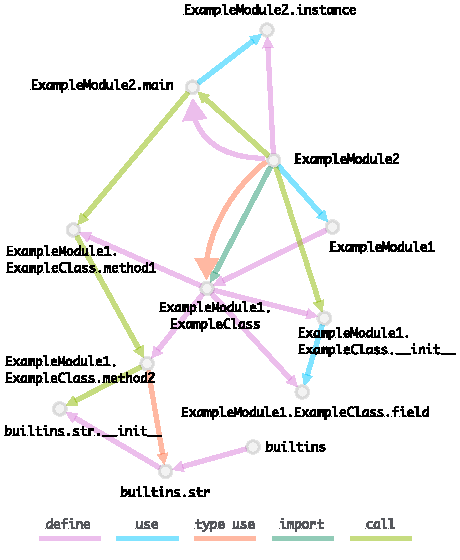
\includegraphics{python_graph_example.pdf}
    \caption{Example of global graph constructed from two toy modules.}\label{fig:python_graph}
\end{figure}

\begin{table}[]
\centering
\begin{tabular}{lll}
    \toprule
    Node Type        & Count  \\ \midrule
    Function        & 221822 \\ \midrule
    Class field     & 83077 \\ \midrule
    Class           & 35798 \\ \midrule
    Module          & 18097 \\ \midrule
    Class method    & 14953 \\ \midrule
    Non-indexed symbol  & 853  \\ \bottomrule
\end{tabular}
\caption{Node types present in Python source graph\label{tbl:python_node_count}}
\end{table}

\begin{table}[]
\centering
\begin{tabular}{ll}
\toprule
Edge Type       & Count \\ \midrule
Call            & 614621 \\ \midrule
Define/Contain  & 431115 \\ \midrule
Type use        & 239543 \\ \midrule
Import          & 121752 \\ \midrule
Inherit         & 26525 \\ \bottomrule
\end{tabular}
\caption{Edge count in Python graph by edge type\label{tbl:python_edge_count}}
\end{table}

\subsection{Description of Learning Objectives}

% In this paper, we pursue several goals. First, we are studying global graph representation for the source code. We do this by evaluating a GNN model trained on this graph on several tasks. 
One of our goals is to evaluate a GNN model trained on a global source graph. We do this by training this model using several objectives.

The first objective is SCO \textbf{name prediction}, which includes predicting function names, class names, variable names, etc. This objective can be seen as semantically challenging because the original graph contains only the information about the relationships between SCOs. The premise for this task is that objects with specific common names have fixed usage patterns. The fact that some objects can be references in common settings implies that they have a similar purpose, and often, similar names. In this task, the target can be defined for every node in the global graph.

The second objective is \textbf{predicting names of variables} that are used inside a function. This is also a semantically challenging task. Very often, variable names explain the purpose of a function, or at very least, the topical area to which this function belongs. We expect that functions that implement similar functionality, or belong to the same package are likely to use similar variable names. The variable names are extracted from function bodies. Because of the way the objective is specified, the target is defined only for the nodes in the graph that represent functions.  

The third objective is \textbf{predicting next function} to be called after the current function. In order to be able to predict the next call, the model should learn common usage patterns for functions. These usage patterns include built-in functions, functions from the same package, and functions from other packages. As with the case of variable name prediction, the objective is defined only for the nodes that represent functions. 

Some of the objectives are defined only for a subset of nodes. However, the GNNs are implemented in a way, where representation for all nodes are trained simultaneously. For this reason, GNN learning tasks are sometimes seen as semi-supervised learning problems.

All of three objectives can be treated as link prediction problems. During the training, embeddings for two nodes are passed to the classifier for link prediction. The two nodes specify the source and destination of a directed edge. Depending on the objective, the two nodes are taken from different groups. The source node always represent an SCO object in the global graph, and its embedding is computed using GNN\@. The second node can be either a node for SCO name, a node for the variable name, or another SCO\@. In the case of names, the embedding for the second node is drawn form a dedicated embedding table. Otherwise, it is also generated by GNN\@. The link prediction is implemented by concatenating the embeddings for the source and destination of the edge, and passing the resulting vector to a binary classifier. We implement this classifier using a simple neural network.

We use three objectives explained above to train several GNN models to see to which extent the information about global relationships is useful for solving these tasks. Moreover, we experiment with a multitask objective. After, we investigate the applicability of learned distributed representations to predict properties of some of the nodes in the global graph with a series of experiments. These experiments are designed to identify the usefulness of objectives described above for solving other tasks. The details of these experiments are given in XXX.

\subsection{GNN Models}

Graph Neural Networks (GNN) is based on a message-passing mechanism. Each node possesses an internal state. During message-passing, the node sends its state to its neighbors. The neighbors aggregate messages from adjacent nodes using a neural network. Usually, the messages are passed over the entire network a fixed number of steps. The message-passing steps are treated as network layers. The final node state is passed to the classifier that predicts links. The initial representation of a node is a context-free embedding. Embeddings from the consecutive layers can be viewed as the contextual. The size of the context depends on the number of layers. The best context size for solving the link prediction task is subject to exploration.

In our experiments, we use two different GNN architectures. The first is the Graph Attention Network (GAT). This architecture does not support different types of relationships and treats them the same. The second architecture is Relations Graph Convolutional Network (RGCN). This network was designed to process heterogeneous graphs and supports different types of edges. We use these two types of networks to investigate the impact of the edge types on the final result. 

Other works that rely on GNNs use more complicated architectures \cite{Allamanis2017} \cite{Cvitkovic2018}. However, the search of the best neural architecture is not our goal. For the latest findings in the area of architecture search for processing source code with GNNs see \cite{hellendoorn2020global}.

The reason we choose GNN models for our experiments is because, at the moment, they are considered the most suitable for processing graphs. 
We tried to use other approaches for learning representations for nodes, specifically Node2Vec, but they did not prove to be useful for out tasks.

% \textbf{Graph Attention Network} is a model that uses the attention mechanism during the aggregation of messages. Thus, this neural network can select the most relevant messages for computing the current internal state.

% $$
% h_i^{(l+1)}=\sigma\left(\sum_{j\in \mathcal{N}(i)} {\frac{1}{c_{ij}} W^{(l)}h^{(l)}_j}\right)
% $$

% \textbf{Relational Graph Convolutional Network} allows modeling heterogeneous graphs with different relation types. In this variant, there is a dedicated set of weights for each type of connection. 
% $$
% h_i^{(l+1)} = \sigma\left(\sum_{r\in \mathcal{R}}
% \sum_{j\in\mathcal{N}_r(i)}W_r^{(l)}h_j^{(l)}\right)
% $$


\section{\uppercase{GNN Training Procedure}}

In the process of training a GNN model on one of the objectives, embeddings for graph nodes are learned. These embeddings are used in several scenarios. First, they are passed to the classifier that predicts links for the main objective. Second, they are used in further experiments with transfer learning. Because of this setting, the optimization of the main objective can be seen as the pre-training step. The assessment of transfer learning requires training additional models on parts of the same graph.

Due to the need to evaluate the usefulness of the learned embeddings for the transfer learning, a careful pre-processing procedure for splitting data into train and test sets should be used. This procedure helps to ensure that the training signals do not leak into the test data. In this section, we are going to explain:
\begin{itemize}
    \item The pre-processing procedure for the global graph
    \item What is the train-test splitting policy for training the main objective
    \item How does pre-training procedure looks
    \item What is the list of experiments for assessing the transferability of learned embeddings
\end{itemize}

The entire training and testing procedure is shown in the Figure XXX.

\subsection{Dataset Splits for Training and Evaluation}

The global graph is prepared in the following way:
\begin{enumerate}
    \item Edges are split into the train set and holdout set. The holdout set is used in future experiments. Without a holdout set, the results of future experiments may be biased. After removing holdout edges from the main graph, the disconnected nodes are filtered, so that the graph remains connected. The fraction of the holdout edges is 10\% of the total.
    \item Training objectives will be defined based on node embeddings. For this reason, the train, test, and validation sets are creating splitting on nodes. The test set is used in future experiments for training and testing. Validation and test sets are equal in size and constitute 40\% of all nodes.
\end{enumerate}

\subsection{GNN Training Procedure}

As it was mentioned above, the nodes are split into three groups: train, validation and test sets. As it was described in XXX, the goal is to predict the presence of a link between the source and destination nodes. During the training, only positive samples are available in the dataset. The negative samples are generated randomly. When preparing a batch for training, we take source nodes from the train set. Then, we sample the positive edges that are available for these nodes in the global graph. After, we generate negative edges by sampling destination nodes using the negative sampling procedure from~\cite{mikolov2013distributed}. The fact that the graph edges are split into the train and validation sets based on the source node allows link prediction classifier to observe all the connections of a specific node. Then, it can transfer its knowledge onto the edges with source nodes that it has never observed before.

The evaluation of the quality of the model is performed in a similar way. We take nodes from the validation set, and take all positive edges for these nodes. In addition, we generate negative edges using negative sampling procedure describe above. The number of positive and negative samples is equal. We assess the quality of the model using accuracy. This way, the accuracy of the random baseline is 0.5.

\section{\uppercase{Experiments for Transfer Learning}}

One of our goals is to study the transferability of learned representations for nodes onto different tasks. For this reason, we use embeddings trained using objectives described in XXX for predicting some of the properties of these nodes. All of the properties are posed as link prediction problems. In fact, the experiments described below help to assess how useful learned node embeddings are for predicting other links in the global graph. The list of experiments include:
\begin{enumerate}
    \item \textbf{Predicting SCO name} 
    This task is the exact copy of one of objectives of the main task. It is expected that is the main objective was to predict SCO names, the experiment should show nearly identical performance. Moreover, this task allows to evaluate whether embeddings trained on predicting next calls are useful for predicting names as well. 
    \item \textbf{Predicting variable name usages}
    The goal of this task is to predict variable names that were used inside a given function.
    \item \textbf{Predicting next function}.
    In this experiment, the task is to predict the edge between functions A and B, that shows that B was called after function A. 
    \item \textbf{Predicting call links}. 
    In this experiment, the goal is to predict the existence of call edges between two nodes. Training data is taken from the holdout set that contains edges that were not used during training. 
    \item \textbf{Predicting type usage}.
    The edges for type use are taken from the holdout edges. These edges show that the specific type (class) was mentioned inside the body of some function. 
    \item \textbf{Predicting node types}.
    In this procedure, a simple node embedding classifier is applied. This procedure does not require to predict interaction between two nodes and needs only one node embedding as an input. In general, any types of labels can be used. We use the types of nodes as a label.
\end{enumerate}

The training procedure for the experiments listed above resembles the procedure for training the main objective that was described in XXX. The experiments are performed only on nodes that were previously reserved for the test set. The embeddings for nodes were precomputed previously using GNN and now are retrieved using an embedding table. The embeddings for the SCO nodes remain unchanged during the experiments. This ensures that we test what can be extracted from these embeddings instead of using them merely for initialization. 

We take the test set of nodes that was generated during preparation of the main objective. We split this set into the new train and test sets. Then, the SCO embeddings are used for link prediction. It is worth noting that we train embedding for names (including variable names) and the link prediction classifier from scratch. The summary of what is trained for each experiment is shown in Table~\ref{tbl:experiment_desc}.

\begin{table*}
    \centering
    \caption{Description of experiments and what is trained}\label{tbl:experiment_desc}
    \begin{tabular}{|p{3cm}|p{6cm}|p{6cm}|}
    \toprule
        \textbf{Experiment} & \textbf{Model description} & \textbf{What is trained} \\ \midrule
        Next function, call, type use & Both nodes are from the original graph. Node embeddings are concatenated and classified & Binary classifier that predicts the the presence of edge between nodes \\ \midrule
        Function name, variable names & Src node from the original graph, dst node is new. Node embeddings are concatenated and classified & Binary classifier that predicts the presence of edge between nodes. Embeddings for dst noes. \\ \midrule
        Node type & Node is classified into a relatively small number of classes. Node embedding taken from the original graph. & Node classifier \\ \bottomrule
    \end{tabular}
\end{table*}



\section{\uppercase{Experimental Setup and Results}}


\section{\uppercase{Discussion}}

\subsection{Splitting on nodes or edges}

There should be no (significant) leak of training signals from the train to the test set. The src nodes appear either in the train or in test sets. If node A is from the train set, node B is from the test set, and C is a common target, then edge A->C is used for training, B->C used for testing. But in future experiments embedding for C is trained from scratch, so there should be no leak.

There are two ways to handle training data for the experiment. Most of the experiments can be seen as binary classification problem, that makes a decision whether an edge between two nodes exist. In these experiments src nodes are always a part of the original graph, and dst nodes sometimes can be some new nodes. The training data is given as a list of edges. There are two approaches to split this data into train and test set. The first, and the most evident approach, is to split edges into two groups. The second approach is to split the edges based on their src node. That is, use the edges with some src nodes only to train test, and the rest - in test set. 
We argue that the second approach can give more information to the classifier about how to interpret the embeddings of the nodes from the original graph. When the edges are simply split into two groups, the some edges that share a common src node can appear in both train and test splits. This way, the classifier can struggle to predict some of the edges, because only the partial knowledge was present in the training set. However, when the split is performed on the basis of src nodes, the classifier has the opportunity to see how a node with a given embedding is connected to other nodes, and learn how to extract useful information from this embedding. 

\subsection{The need for multiple splits}

A natural question is why all of these complicated data splits necessary. In this work we are using a GNN model to train node embeddings. These models implement message passing procedure. For this reason, GNN models are sometimes considered as semi-supervised. All the data is present in the same graph, and training signals naturally affect even unlabeled nodes. For this reason it is hard to make conclusions about the transferability of the learned embeddings. Moreover, the real datasets are rarely complete. By introducing several data splits and holdout sets we emulate the data incompleteness. This way we can show that even when trained on incomplete graph, the node embeddings can still be useful.

\subsection{The choice of negative sampling strategy}

Distribution and parameter

\subsection{Evaluation approaches}

We have two types of models. THe first type is used for node classification and has a very small number of target classes. We use accuracy to evaluate the quality of such models. The second type of model tries to decide whether there is an edge between two nodes. In essence, this model solves a binary classification problem. In order to evaluate this model, we take all the positive edges in the test split, and generate an equal amount of the negative edges. The equal proportion of the edges hints that the random baseline for accuracy should be around 0.5. However, this baseline is not relevant in our case for a couple of reasons. First, our goal is to evaluate embeddings. When we train a classifier, it will fit to the current embeddings. Because the target nodes are shared between training and testing edges, it is likely to see the accuracy above 0.5 after fitting the classifier. Second, our negative edges are randomly generated. There is a slight possibility that the generated edge is a good candidate to be a positive edge. To account for this, we conduct the same experiments with node embeddings randomly initialized, and use the resulting score as the random baseline.
For models that have a large amount of target labels, it makes sense to use ranking measures. 

\subsection{Hyperparameter search}


\bibliographystyle{apalike}
{\small
\bibliography{Splash2020.Vitaly}}

\end{document}

